\documentclass{standalone}
\usepackage{tikz}
\usetikzlibrary{shapes.geometric, arrows}

%Inicio del preambulo

\tikzstyle{startstop} = [rectangle, rounded corners, minimum width=3cm, minimum height=1cm,text centered, draw=black, fill=red!30]
\tikzstyle{io} = [trapezium, trapezium left angle=70, trapezium right angle=110, minimum width=3cm, minimum height=1cm, text centered, draw=black, fill=blue!30]
\tikzstyle{process} = [rectangle, minimum width=3cm, minimum height=1cm, text centered, draw=black, fill=orange!30]
\tikzstyle{decision} = [diamond, minimum width=3cm, minimum height=1cm, text centered, draw=black, fill=green!30]
\tikzstyle{arrow} = [thick,->,>=stealth]

%Fin del preambulo

\begin{document}

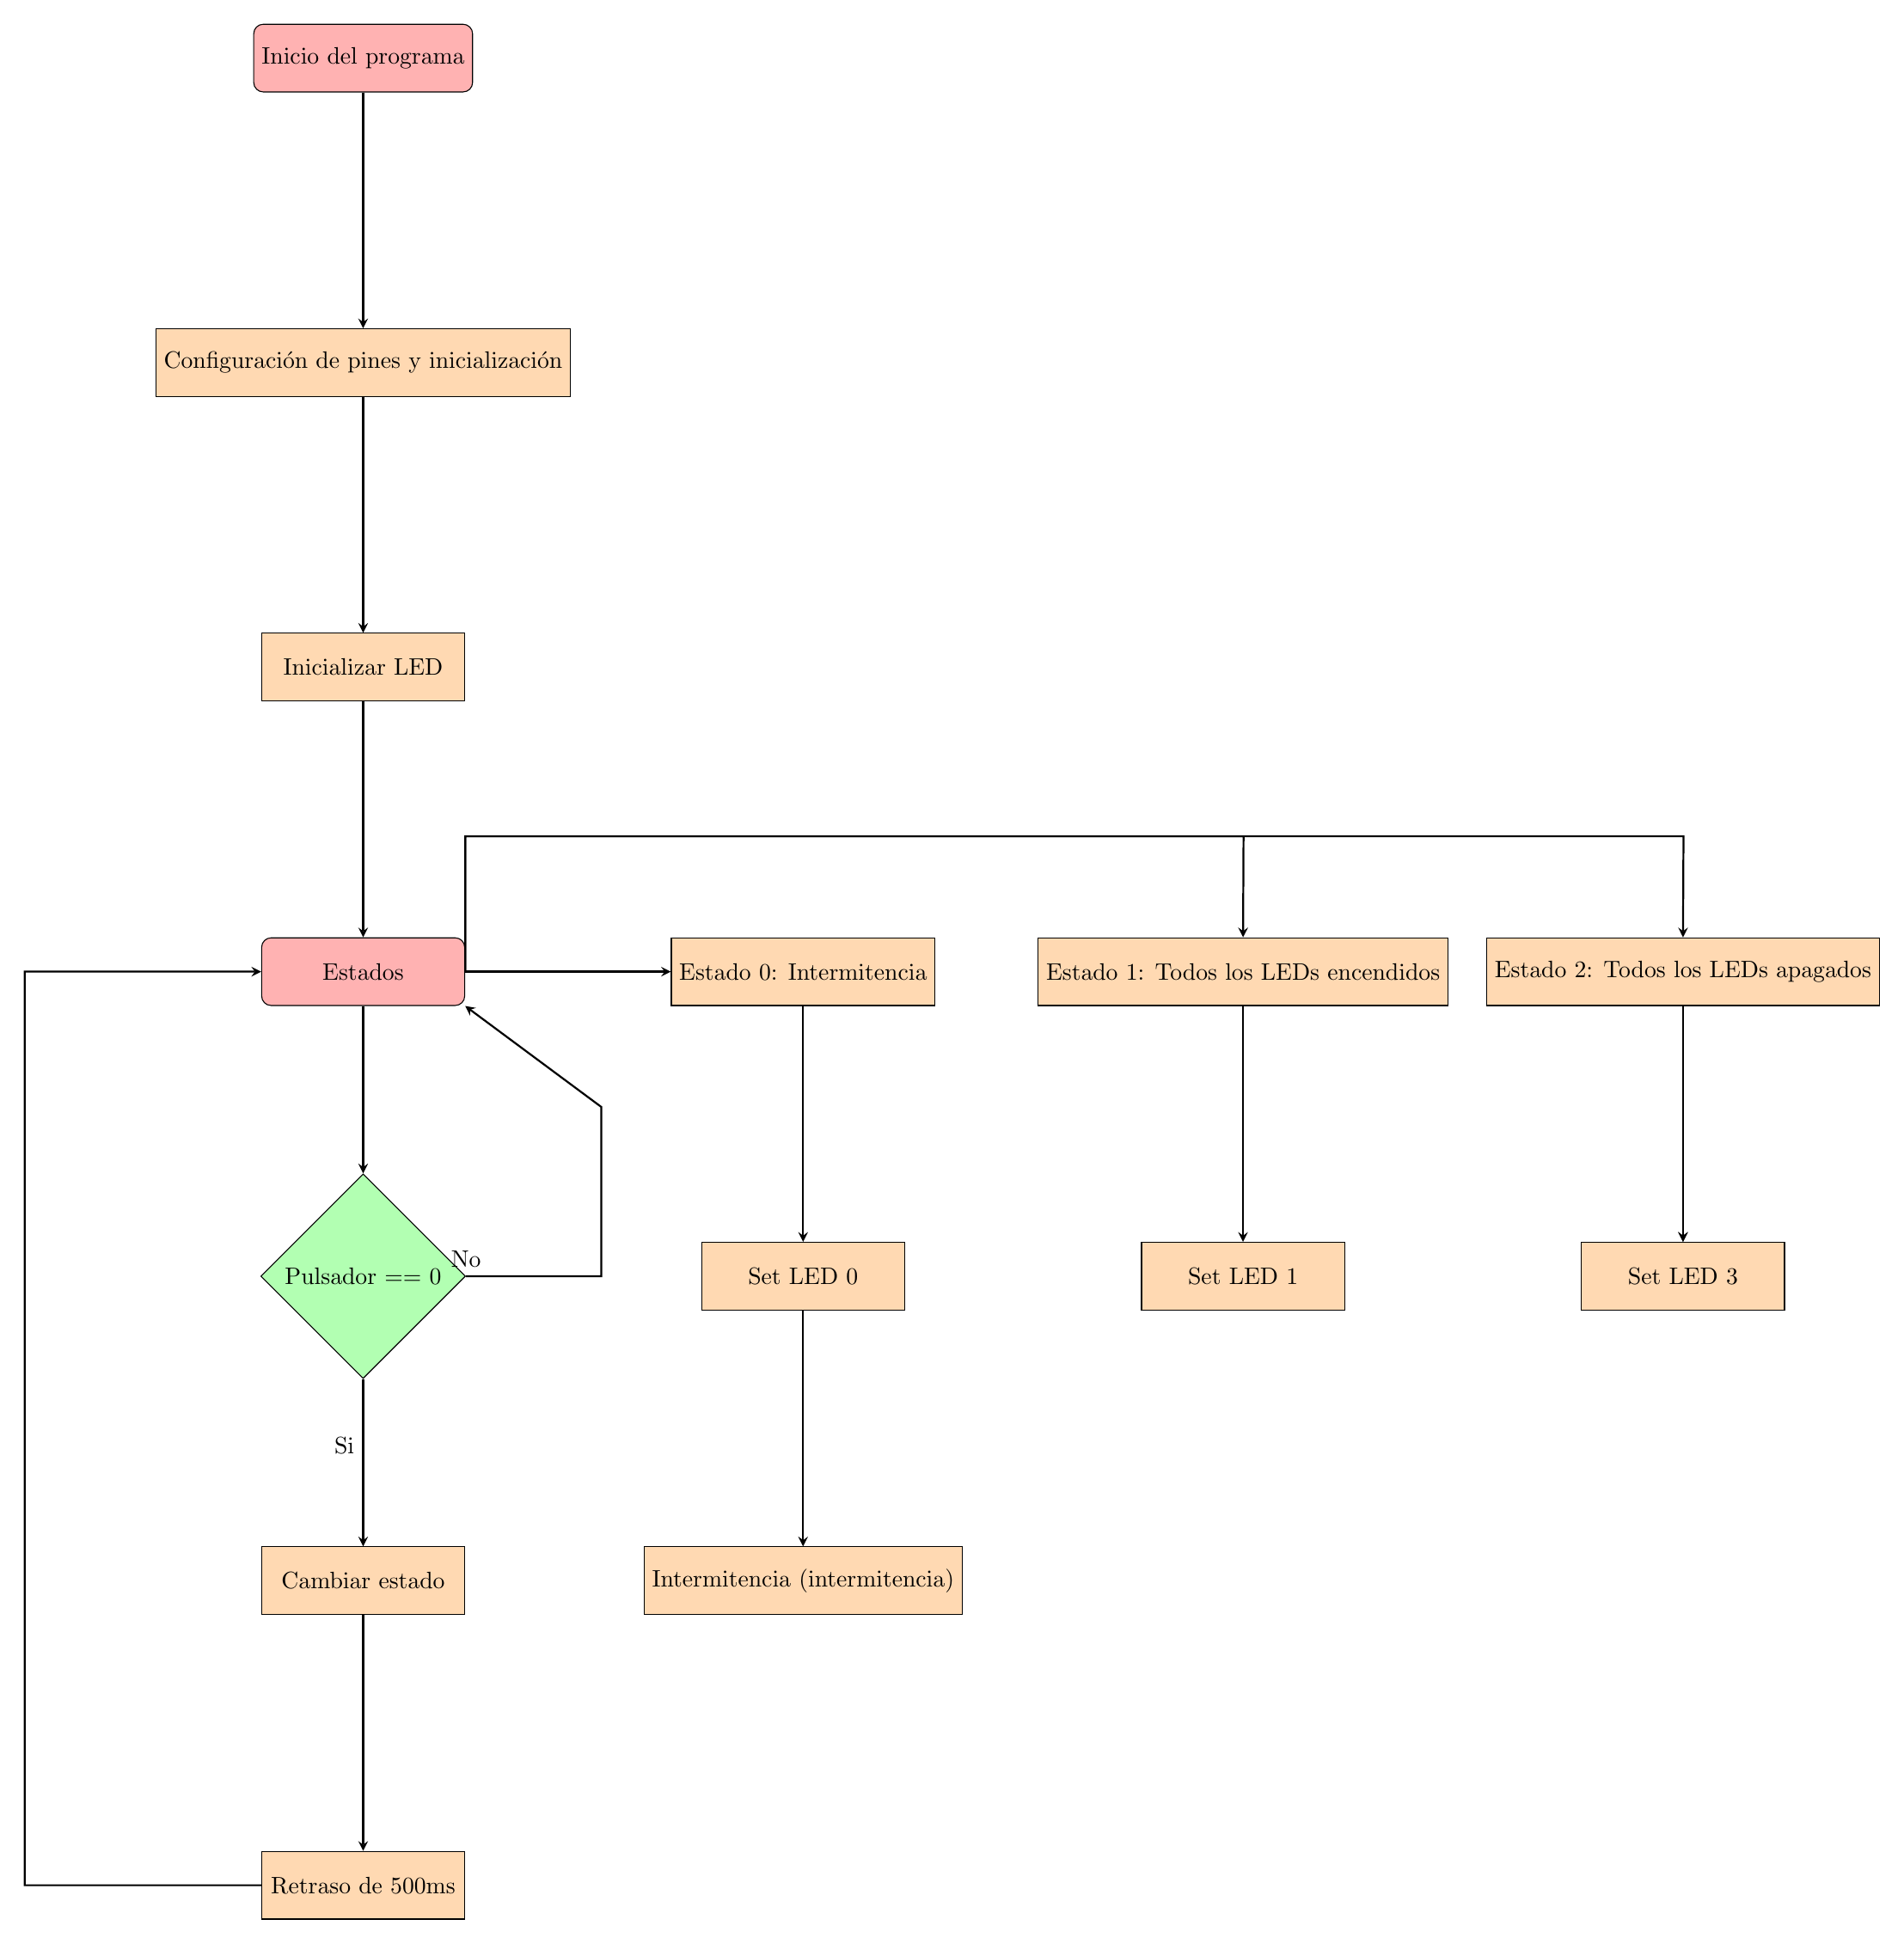
\begin{tikzpicture}[node distance = 4.5cm]
  \node (start) [startstop] {Inicio del programa};
  \node (config) [process, below of = start] {Configuración de pines y inicialización};
  \node (init_leds) [process, below of = config] {Inicializar LED};
  \node (loop) [startstop, below of = init_leds] {Estados};
  %\node (primero) [circle,draw] {1};
  
  \node (estado0) [process, right of = loop, xshift=2cm] {Estado 0: Intermitencia};
  \node (estado1) [process, right of = estado0, xshift=2cm] {Estado 1: Todos los LEDs encendidos};
  \node (estado2) [process, right of = estado1, xshift=2cm] {Estado 2: Todos los LEDs apagados};
  
  \node (set_led0) [process, below of = estado0] {Set LED 0 };
  \node (set_led1) [process, below of = estado1] {Set LED 1 };
  \node (set_led2) [process, below of = estado2] {Set LED 2 };
  \node (set_led3) [process, below of = estado2] {Set LED 3 };
  
  \node (intermitencia) [process, below of = set_led0] {Intermitencia (intermitencia)};
  
  \node (pulsador) [decision, below of = loop] {Pulsador == 0};
  \node (cambiar_estado) [process, below of = pulsador] {Cambiar estado};
  \node (retraso) [process, below of = cambiar_estado] {Retraso de 500ms};
  
  \draw[arrow] (start) -- (config);
  \draw[arrow] (config) -- (init_leds);
  \draw[arrow] (init_leds) -- (loop);
  
  \draw[arrow] (loop) -- (estado0);
  \draw[arrow] (loop.east) --++(0,2) --++(11.5,0) -- (estado1.north);
  \draw[arrow] (loop.east) --++(0,2) --++(18,0) -- (estado2.north);
  
  \draw[arrow] (estado0) -- (set_led0);
  \draw[arrow] (estado1) -- (set_led1);
  \draw[arrow] (estado2) -- (set_led2);
  \draw[arrow] (estado2) -- (set_led3);
  
  \draw[arrow] (set_led0) -- (intermitencia);
  
  \draw[arrow] (loop) -- (pulsador);
  \draw[arrow] (pulsador) --node[anchor=south east]{Si} (cambiar_estado);
  \draw[arrow] (cambiar_estado) -- (retraso);
  \draw[arrow] (retraso) --++(-5,0) --++ (0,13.5) -- (loop.west);
  
  \draw[arrow] (pulsador.east) node[anchor=south]{No} --++(2,0)--++ (0,2.5)-- (loop.south east);
\end{tikzpicture}

\end{document} 